% =============================================================
% Capitulo 9 - Descripcion del modelo experimental
% =============================================================
\chapter{Descripción del modelo experimental}
\label{cap:modelo_experimental}

En los capítulos precedentes se desarrollaron por separado el circuito de detección de picos, la selección del microcontrolador, el diseño del circuito impreso, el \emph{firmware} embebido y el software de supervisión. El presente capítulo describe el conjunto ya integrado y en condiciones de operación: cómo quedó montado el modelo sobre el instrumento, qué funciones expone al operador, cuál es el procedimiento de puesta en marcha, qué ensayos se realizaron sobre el sistema HSRL del Observatorio de Pilar y qué limitaciones conserva el prototipo.

\section{Integración del sistema}
\label{sec:me-integracion}

El modelo experimental está constituido por tres elementos que operan de forma solidaria: la placa de control descrita en el Capítulo~\ref{cap:placacontrol}, el \emph{firmware} residente en el microcontrolador desarrollado en el Capítulo~\ref{cap:firmware} y la interfaz de supervisión del Capítulo~\ref{cap:software_hmi} ejecutada en la computadora del nodo.

\begin{figure}[htpb]
      \centering
      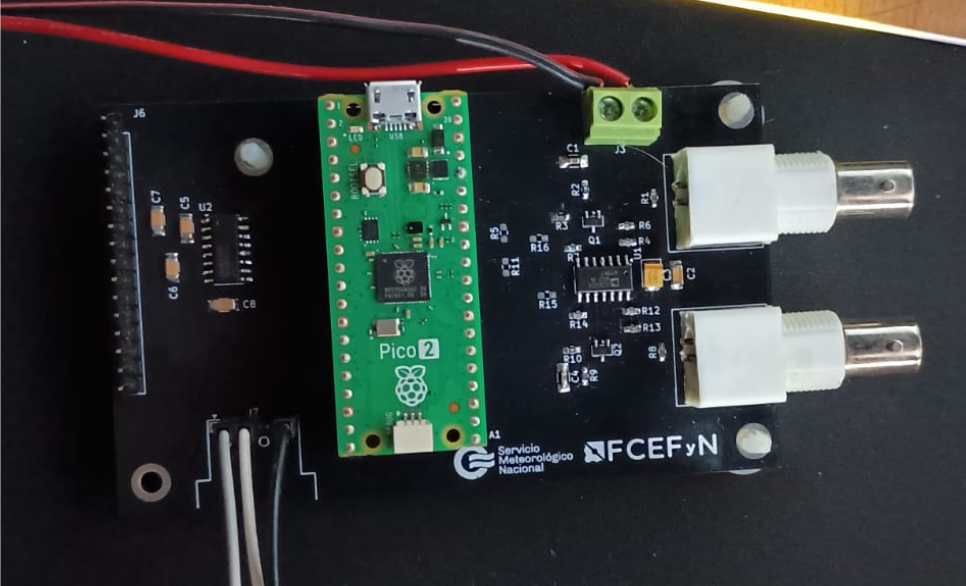
\includegraphics[width=0.7\textwidth]{figuras/9_prototipo.png}
      \caption{Placa de control ensamblada (Fuente: elaboración propia).}
      \label{fig:placaarmada}
\end{figure}

La placa de control reúne en una única pieza los dos canales de detección de picos correspondientes a las señales $P_+$ y $P_-$, el módulo Raspberry Pi Pico~2 montado sobre conectores hembra de $2\times20$ pines y el transceptor MAX3232 con su conector DB9. La alimentación ingresa por una bornera doble de $+12$~V y masa, y las entradas analógicas se materializan mediante conectores BNC ubicados sobre el borde contiguo a los amplificadores.

Para su emplazamiento definitivo, el conjunto se fijó sobre un panel de acrílico montado en el frente del equipo, de modo que los conectores de entrada, el enlace serie hacia el \emph{seeder} y el puerto USB hacia la computadora de control quedaran accesibles. Esta disposición concentra en un único plano frontal todos los puntos de conexión del lazo de sintonización: las salidas de los amplificadores de transimpedancia de los cuatro fotodetectores, las dos entradas para las señales $P_+$ y $P_-$ y el puerto USB.

\begin{figure}[htpb]
      \centering
      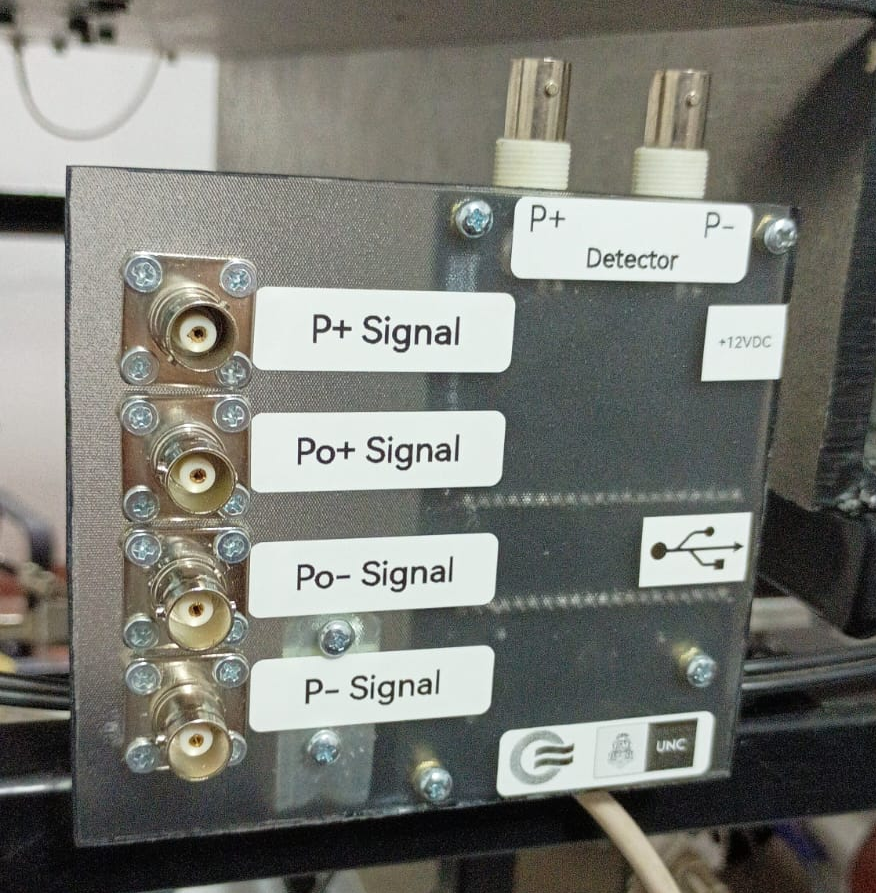
\includegraphics[width=0.7\textwidth]{figuras/9_panelacrilico.png}
      \caption{Panel de acrílico sobre el cual se encuentra montada la placa de control y bornes de salida del TIA (Fuente: elaboración propia).}
      \label{fig:panel}
\end{figure}

La señal de sincronismo del láser \emph{host} se toma del mismo y se adapta al rango lógico del microcontrolador mediante el divisor resistivo descrito en el Capítulo~\ref{cap:micro}. La comunicación con el láser \emph{seeder} se establece por el enlace RS-232 a través del conector DB9. Finalmente, el vínculo con la computadora de supervisión se realiza por USB, sobre el cual el \emph{firmware} expone una consola en modo CDC. Ninguna de estas interfaces exige modificar el camino óptico ni la electrónica de detección original del instrumento, lo que permite revertir la instalación y regresar a la configuración anterior sin intervención adicional.

\section{Funcionalidad del conjunto}
\label{sec:me-funcionalidad}

El sistema cumple, sobre el instrumento montado, las funciones que se enuncian a continuación.

\begin{itemize}
  \item El microcontrolador digitaliza el valor retenido por el detector de picos del canal que corresponda, alternando entre $P_+$ y $P_-$ en disparos consecutivos. El número de picos promediados por canal es configurable en caliente.
  \item El \emph{firmware} calcula el cociente entre ambos canales y corrige el punto de consigna de temperatura del calefactor del \emph{seeder} según la ley de control por histéresis con banda muerta multiplicativa descrita en la Sección~\ref{sec:fw-control}, manteniendo la longitud de onda del láser sobre la línea de absorción del iodo.
  \item Los modos de barrido en lazo abierto recorren el rango útil de temperatura mientras la interfaz registra los mínimos de cada canal, lo que permite localizar el punto de operación.
  \item La secuencia descrita en la Sección~\ref{sec:hmi-auto} encadena cuatro pasos individuales: la detención del barrido, la escritura del punto medio entre los mínimos, la espera de estabilización térmica y el cierre del lazo o sintonización, sin intervención directa del operador.
  \item El \emph{setpoint} se mantiene acotado al intervalo $[h_{\min}, h_{\max}]$ declarado en el \emph{firmware}; si el barrido lo excede, el controlador invierte el sentido y anula la sintonía del \emph{seeder}.
  \item La interfaz presenta el estado del enlace, el estado de las escrituras protegidas, la condición de \emph{second mode} del \emph{seeder} y las amplitudes medidas en función de la temperatura, visualizadas en la Figura~\ref{fig:tandem}, junto con la banda de alarmas jerarquizada de la Sección~\ref{sec:hmi-alarmas}, si es que existen alarmas activas.
  \item Cada sesión genera un archivo completo de operación y un archivo CSV con una fila por ciclo de control, según el contrato de columnas establecido en la Sección~\ref{sec:fw-log}.
\end{itemize}

\begin{figure}[htpb]
      \centering
      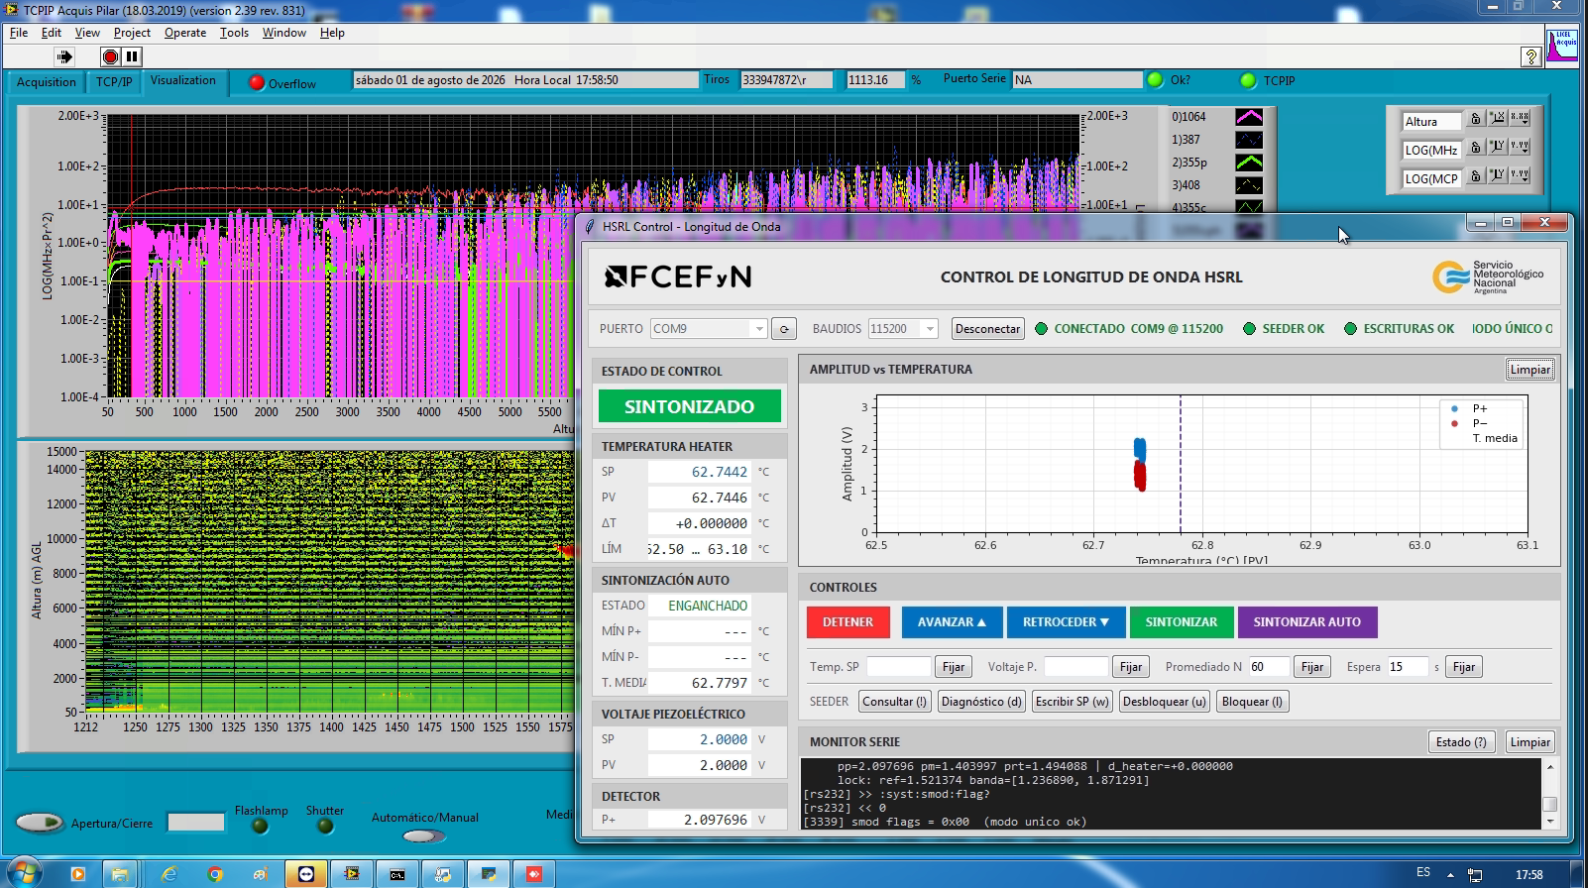
\includegraphics[width=0.7\textwidth]{figuras/9_tandem.png}
      \caption{Software de control de lidar (LABView) operando en conjunto con la HMI implementada (Fuente: elaboración propia).}
      \label{fig:tandem}
\end{figure}

Corresponde señalar que el lazo de control reside íntegramente en el microcontrolador. La interfaz de supervisión actúa como observador y como emisor de comandos, pero no forma parte del lazo: si la computadora se desconecta o el programa se cierra, el \emph{firmware} continúa sosteniendo la sintonización. Esta propiedad es la que habilita la operación desatendida planteada en la Sección~\ref{sec:formulacion_problema}.

\section{Instrucciones de operación}
\label{sec:me-manual}

\subsection{Organización de la pantalla}

La interfaz, cuyo aspecto se muestra en la Figura~\ref{fig:hmiopus}, distribuye el contenido en cuatro zonas siguiendo la jerarquía de pantallas descrita en la
Sección~\ref{sec:isa101}.

\begin{itemize}
      \item La \textbf{barra superior} concentra el establecimiento del enlace (selector
        \textbf{PUERTO}, selector \textbf{BAUDIOS} y botón \textbf{Conectar}) junto a
        los cuatro indicadores permanentes de estado: enlace USB, respuesta del
        \emph{seeder}, habilitación de las escrituras y condición de \emph{second mode}.
      \item La \textbf{columna izquierda} agrupa los valores del proceso en bloques:
        \textbf{ESTADO DE CONTROL}, que informa el modo vigente con un indicador de
        gran tamaño; \textbf{TEMPERATURA HEATER}, con el \emph{setpoint} (SP), la
        temperatura medida (PV), su diferencia ($\Delta T$) y el límite de seguridad
        alcanzado (LÍM); \textbf{SINTONIZACIÓN AUTO}, con los mínimos registrados de
        cada canal y la temperatura media resultante; \textbf{VOLTAJE
        PIEZOELÉCTRICO}; \textbf{DETECTOR}, con las amplitudes $P_+$, $P_-$ y su
        cociente; y \textbf{SINTONIZACIÓN}, con la referencia y la banda muerta
        vigentes.
      \item El \textbf{gráfico central} representa la amplitud de ambos canales en
        función de la temperatura, con una línea vertical que marca la temperatura
        media entre los mínimos. El botón \textbf{Limpiar} descarta los puntos
        acumulados.
       \item El \textbf{panel de control} reúne los cinco botones de modo, los campos de parámetro con su botón \textbf{Fijar} y la fila de comandos dirigidos al \emph{seeder}. Debajo, el \textbf{MONITOR SERIE} reproduce la terminal de la sesión y admite el envío de comandos sueltos.
\end{itemize}

La correspondencia entre cada control y la acción que ejecuta se resume en la
Tabla~\ref{tab:me-controles}. Entre paréntesis se indica el comando equivalente del
\emph{firmware} (Sección~\ref{sec:fw-consola}), de modo que toda operación puede
realizarse también desde el monitor serie si la interfaz no estuviera disponible.

\begin{table}[htpb]
\centering
  \begin{tabular}{@{}p{0.30\textwidth}p{0.62\textwidth}@{}}
  \toprule
  \textbf{Control} & \textbf{Acción} \\
  \midrule
  \multicolumn{2}{@{}l}{\textit{Modos de operación}} \\
  \textbf{DETENER} (\texttt{s})   & Interrumpe el barrido y la sintonización. Deja el \emph{setpoint} en su último valor. \\
  \textbf{AVANZAR} (\texttt{f})   & Barrido ascendente en lazo abierto, aplicando el paso grueso en cada ciclo. \\
  \textbf{RETROCEDER} (\texttt{b})& Barrido descendente en lazo abierto. \\
  \textbf{SINTONIZAR} (\texttt{g})& Cierra el lazo tomando como referencia el cociente de referencia de dos ciclos atrás. \\
  \textbf{SINTONIZAR AUTO}        & Ejecuta la secuencia completa de la Sección~\ref{sec:hmi-auto}: detiene, escribe la temperatura media, aguarda la estabilización y cierra el lazo. \\
  \midrule
  \multicolumn{2}{@{}l}{\textit{Parámetros (se confirman con \textbf{Fijar})}} \\
  \textbf{Temp. SP} (\texttt{T})      & \emph{Setpoint} del calefactor. \\
  \textbf{Voltaje P.} (\texttt{P})    & Tensión del piezoeléctrico del \emph{seeder}. \\
  \textbf{Promediado N} (\texttt{A})  & Cantidad de picos a promediar por canal. \\
  \textbf{Espera} (\texttt{E})        & Pausa de estabilización térmica al inicio de cada ciclo, en segundos. \\
  \midrule
  \multicolumn{2}{@{}l}{\textit{Comandos al \emph{seeder}}} \\
  \textbf{Consultar} (\texttt{!})     & Lee temperatura y tensión actuales del \emph{seeder}. \\
  \textbf{Diagnóstico} (\texttt{d})   & Consulta el estado de la protección y vacía la cola de errores. \\
  \textbf{Escribir SP} (\texttt{w})   & Fuerza la escritura inmediata del \emph{setpoint} y verifica su aceptación. \\
  \textbf{Desbloquear} (\texttt{u})   & Habilita los comandos protegidos. \\
  \textbf{Bloquear} (\texttt{l})      & Vuelve a proteger los comandos de escritura. \\
  \midrule
  \multicolumn{2}{@{}l}{\textit{Monitor serie}} \\
  \textbf{Estado} (\texttt{?})        & Solicita el envío completo de parámetros y la lista de columnas del registro. \\
  \textbf{Limpiar}                    & Vacía la consola en pantalla, sin afectar los archivos de registro. \\
  \bottomrule
  \end{tabular}
  \caption{Controles de la interfaz y comando equivalente del \emph{firmware} (Fuente: elaboración propia).}
  \label{tab:me-controles}
\end{table}

\subsection{Puesta en marcha}

El procedimiento de arranque es el siguiente:

\begin{enumerate}
  \item Verificar que los conectores BNC de $P_+$ y $P_-$, la entrada de sincronismo y el cable DB9 hacia el \emph{seeder} se encuentren firmemente asentados en el panel frontal.
  \item Verificar la energización de la placa con la fuente de $+12$~V. Cuando el LED se encuentra prendido fijamente el sistema está listo para operar.
  \item Conectar el cable USB a la computadora de supervisión y ejecutar la interfaz mediante el inicio de \texttt{hmi.py}.
  \item Seleccionar el puerto serie correspondiente e iniciar la comunicación mediante el botón \textbf{Conectar}. La barra superior debe indicar el enlace USB establecido, el \emph{seeder} respondiendo y las escrituras habilitadas.
\end{enumerate}

Si el indicador \textbf{ESCRITURAS} señala que los comandos permanecen protegidos,
debe pulsarse \textbf{Desbloquear} antes de intentar cualquier ajuste; en caso
contrario el \emph{seeder} descarta silenciosamente los \emph{setpoints} enviados.

\subsection{Localización del punto de operación}

Con el láser en régimen y el sistema recibiendo pulsos de sincronismo, se ordena un
barrido pulsando \textbf{AVANZAR} o \textbf{RETROCEDER}, según el sentido en que se
desee recorrer el rango de temperatura. El indicador \textbf{ESTADO DE CONTROL} pasa
a señalar el modo activo y el gráfico comienza a poblarse con las amplitudes de
$P_+$ y $P_-$ en función de la temperatura. A medida que avanza el barrido, los
campos \textbf{MÍN P+} y \textbf{MÍN P-} conservan el valor mínimo alcanzado por cada
canal junto con la temperatura a la que se produjo y \textbf{T. MEDIA} muestra el
punto medio resultante.

El barrido debe sostenerse hasta que ambos mínimos hayan quedado registrados,
condición que se verifica observando que las dos curvas del gráfico hayan atravesado
su valle y que \textbf{T. MEDIA} exhiba un valor estable. Si el punto de consigna
alcanza un extremo del rango de seguridad, el \emph{firmware} invierte el sentido del
barrido por sí solo.

\subsection{Sintonización}

Habiendo realizado múltiples barridos, se dispone de dos opciones de sintonización.

El procedimiento automático consiste en pulsar \textbf{SINTONIZAR AUTO}. La interfaz detiene el barrido,
escribe la temperatura media como punto de consigna, fuerza su escritura, aguarda la
estabilización térmica, deja transcurrir cuatro ciclos y recién entonces cierra el
lazo. El avance de la secuencia se sigue en el campo \textbf{ESTADO} del bloque
\textbf{SINTONIZACIÓN AUTO}. Si no hay mínimos registrados, o si la temperatura media
cae fuera del rango declarado por el \emph{firmware}, la secuencia no se inicia y el
motivo aparece en el monitor serie.

El procedimiento manual reproduce los mismos pasos uno a uno: pulsar
\textbf{DETENER}; ingresar la temperatura media en \textbf{Temp. SP} y confirmarla
con \textbf{Fijar}; pulsar \textbf{Escribir SP} para forzar la escritura sin esperar
a que concluya el ciclo en curso; esperar a que \textbf{PV} coincida con el valor de
\textbf{SP} en el bloque \textbf{TEMPERATURA HEATER}; y finalmente pulsar
\textbf{SINTONIZAR}. Conviene esta vía cuando se desea fijar un punto de trabajo
distinto del punto medio, por ejemplo para comprobar el correcto desplazamiento de las líneas de absorción o el camino óptico de los haces.

En ambos casos, el cierre correcto del lazo se reconoce porque \textbf{ESTADO DE
CONTROL} indica el modo de sintonización.

\subsection{Operación en régimen}

Una vez sintonizado el sistema, la operación no requiere intervención. El operador dispone de los siguientes elementos para evaluar el estado del sistema:

\begin{itemize}
  \item La ausencia de la banda de alarmas, que sólo se despliega ante una
        condición activa.
  \item La permanencia del \emph{setpoint} dentro del rango de seguridad, visible
        sobre el eje de abscisas del gráfico y en el campo \textbf{LÍM}.
  \item El indicador \textbf{MODO ÚNICO} de la barra superior, que advierte cuando el
        \emph{seeder} abandona la operación monomodo y las mediciones del ciclo dejan
        de ser representativas.
  \item El campo \textbf{CICLO}, cuyo incremento regular confirma que el
        \emph{firmware} sigue recibiendo pulsos de sincronismo.
\end{itemize}

Ante la indicación de segundo modo, la acción correctiva consiste en ingresar un
nuevo valor en \textbf{Voltaje P.} y confirmarlo con \textbf{Fijar}, hasta restituir
la operación monomodo. El \emph{firmware} informa la condición pero no actúa sobre
ella de manera deliberada, de modo que la decisión queda en el operador.

\subsection{Archivos generados}

Cada ejecución de la interfaz produce dos archivos en la carpeta \texttt{logs/}, nombrados con la misma marca temporal de inicio del HMI: un archivo de texto con la totalidad de los comandos enviados y las líneas recibidas, destinada al análisis de incidentes, y un archivo CSV con una fila por ciclo de control, destinado al análisis de los datos. El encabezado del CSV se construye a partir de los nombres de columna que el propio \emph{firmware} declara, según lo detallado en la Sección~\ref{sec:hmi-registro}.

\subsection{Detención}

Para detener el control se pulsa \textbf{DETENER}, que interrumpe tanto el barrido
como la sintonización y deja el punto de consigna en su último valor. El indicador
\textbf{ESTADO DE CONTROL} pasa a señalar la condición de detenido. Este botón
cancela además cualquier secuencia de sintonización automática en curso, por lo que
opera como parada de emergencia del lazo.

El \emph{seeder} conserva el último \emph{setpoint} aun cuando la placa se
desenergice, de modo que un rearranque posterior parte de una condición conocida. Si
se desea impedir escrituras accidentales antes de retirar el equipo de servicio,
conviene pulsar \textbf{Bloquear} para volver a proteger los comandos de escritura.

\section{Ensayos sobre el sistema HSRL del Observatorio de Pilar}
\label{sec:me-ensayos}

El conjunto se instaló sobre el sistema HSRL del Observatorio Geofísico y Meteorológico de Pilar y se sometió a una serie de ensayos
orientados a verificar su desempeño en condiciones reales de operación.

\subsection{Verificación funcional inicial}

El primer ensayo tuvo por objeto comprobar que el sistema fuera capaz de cambiar el punto de operación y sostenerlo con el instrumento en funcionamiento. Primero se mantuvo fija una temperatura, para determinar el comportamiento del sistema en estado estacionario. El resultado se muestra en la Figura~\ref{fig:stop}, donde se observa que el lazo mantiene la temperatura de consigna en lazo abierto durante un período de 13 horas, sin intervención del operador. Cabe destacar la variación de amplitud en los canales $P_+$ y $P_-$, que se debe a la fluctuación de temperatura en la celda de iodo, puesto que la misma posee un control ON/OFF. Debido a que la temperatura de la celda es proporcional a su absorción, la variación de amplitud en los canales es esperable y no afecta el desempeño del lazo de control.

\begin{figure}[htpb]
      \centering
      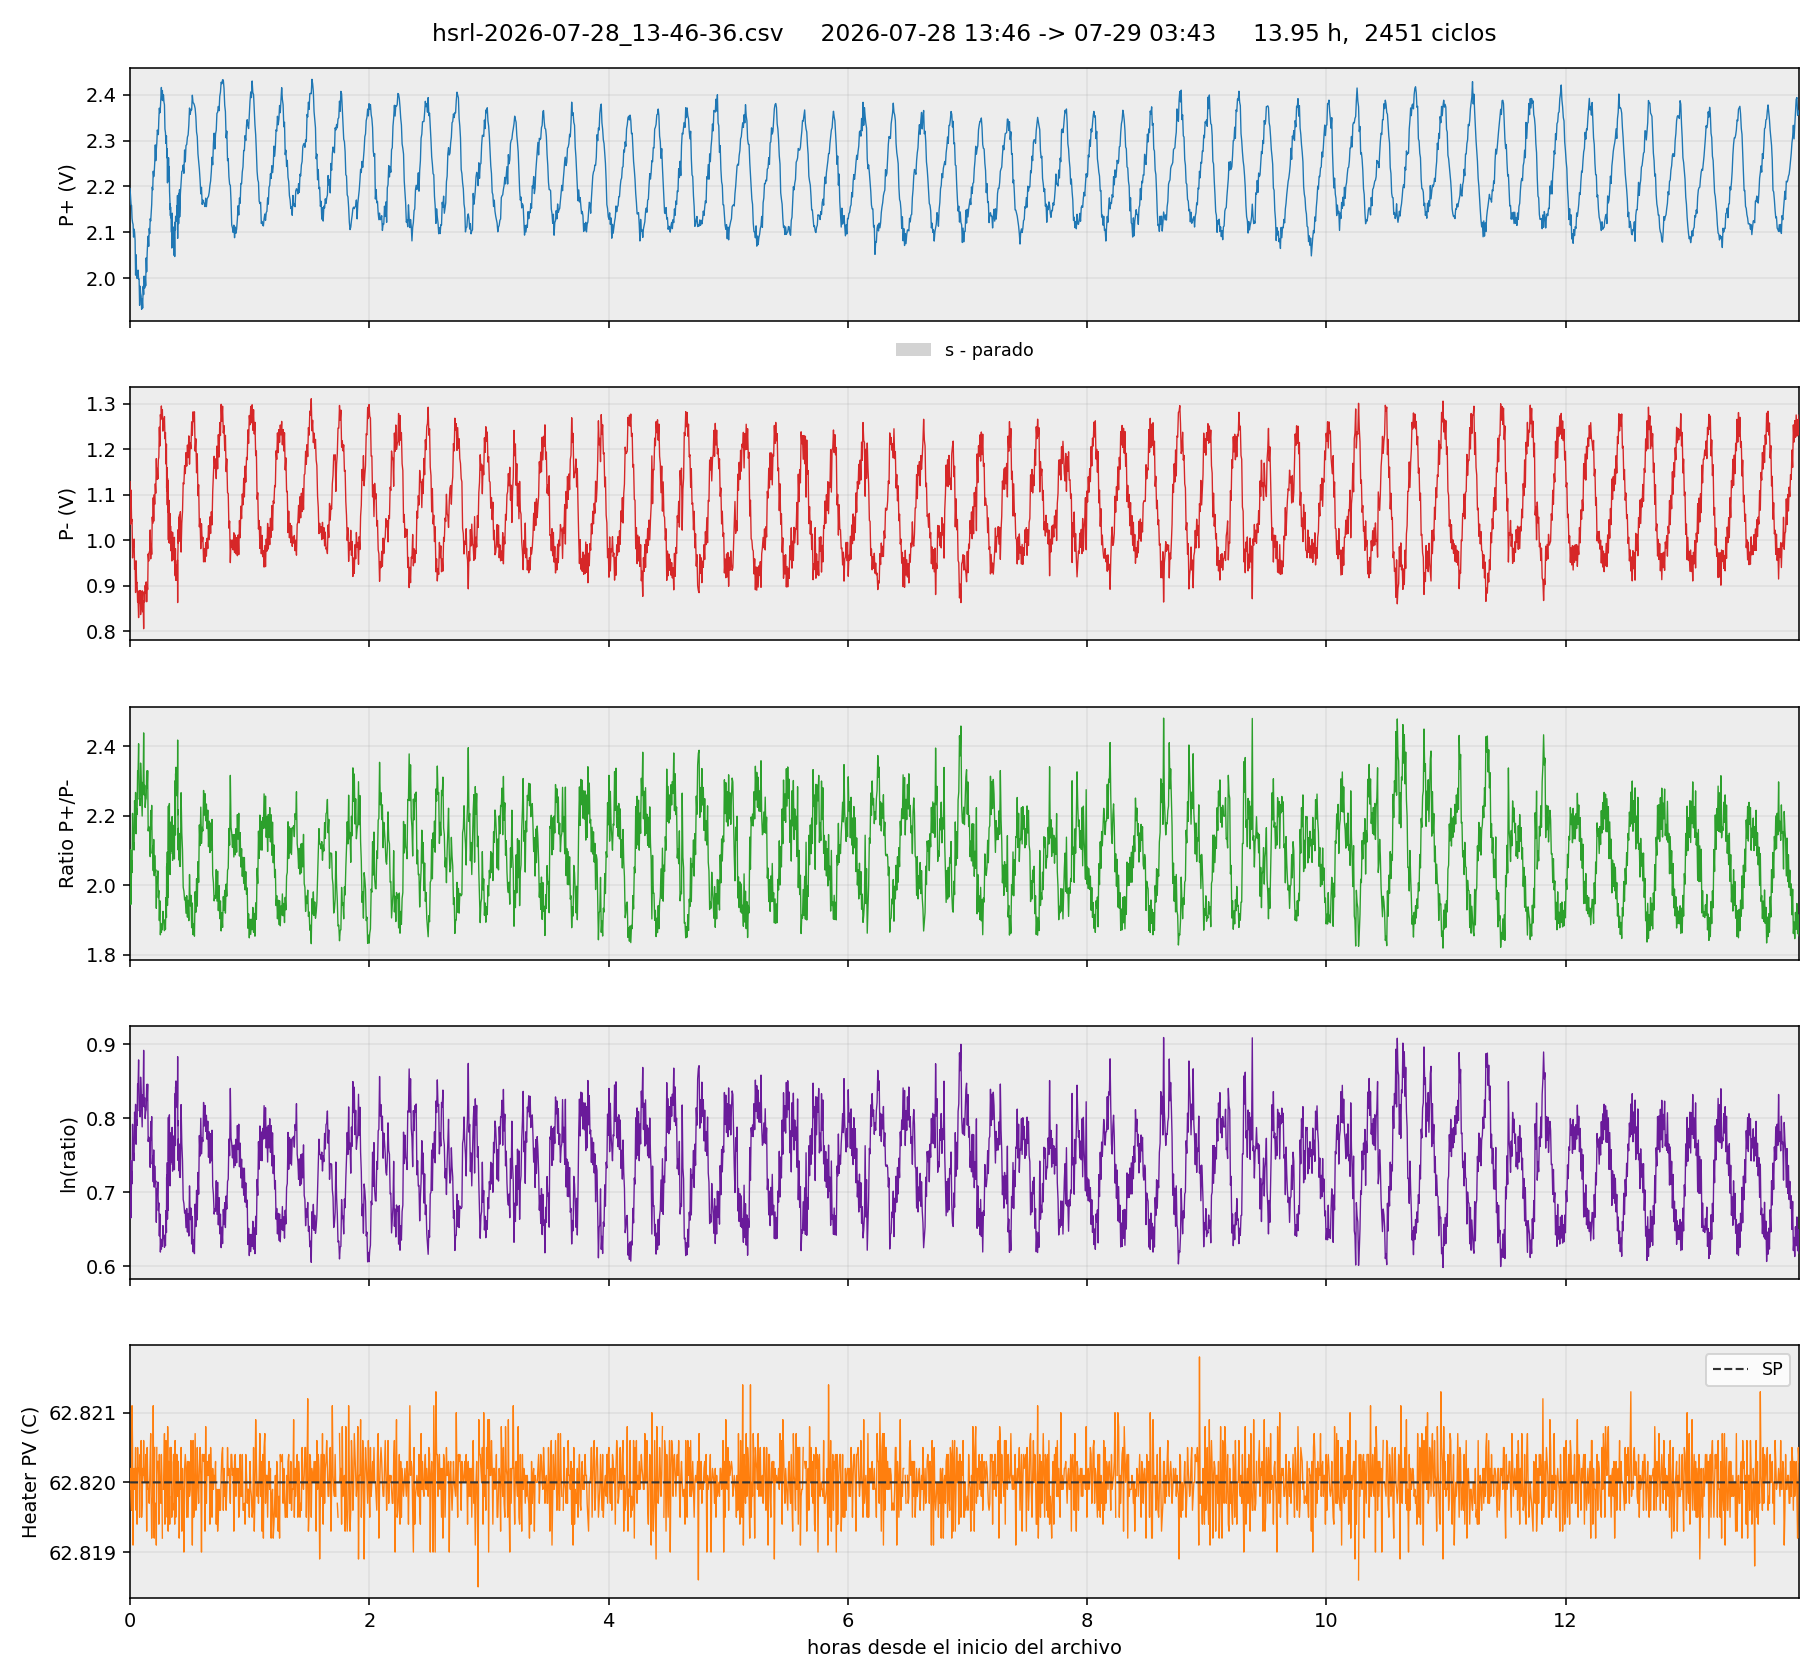
\includegraphics[width=1\textwidth]{figuras/9_stop.png}
      \caption{CSV generado por la HMI, luego de mantener fija una temperatura de 62,82\,\textcelsius\ durante 13 horas (Fuente: elaboración propia).}
      \label{fig:stop}
\end{figure}

Luego de verificar la correcta operación para selección de temperatura a lazo abierto, se iniciaron sucesivos barridos de temperatura, ilustrados en la Figura~\ref{fig:sweep}. En cada barrido se registraron los mínimos de cada canal y se determinó el punto medio entre ambos, que constituye el punto de trabajo para el cierre del lazo. La Figura~\ref{fig:sweep} muestra un barrido de temperatura de 62,3\,\textcelsius\ a 63,1\,\textcelsius, donde se observa la variación de las señales $P_+$ y $P_-$ con la temperatura.

\begin{figure}[htpb]
      \centering
      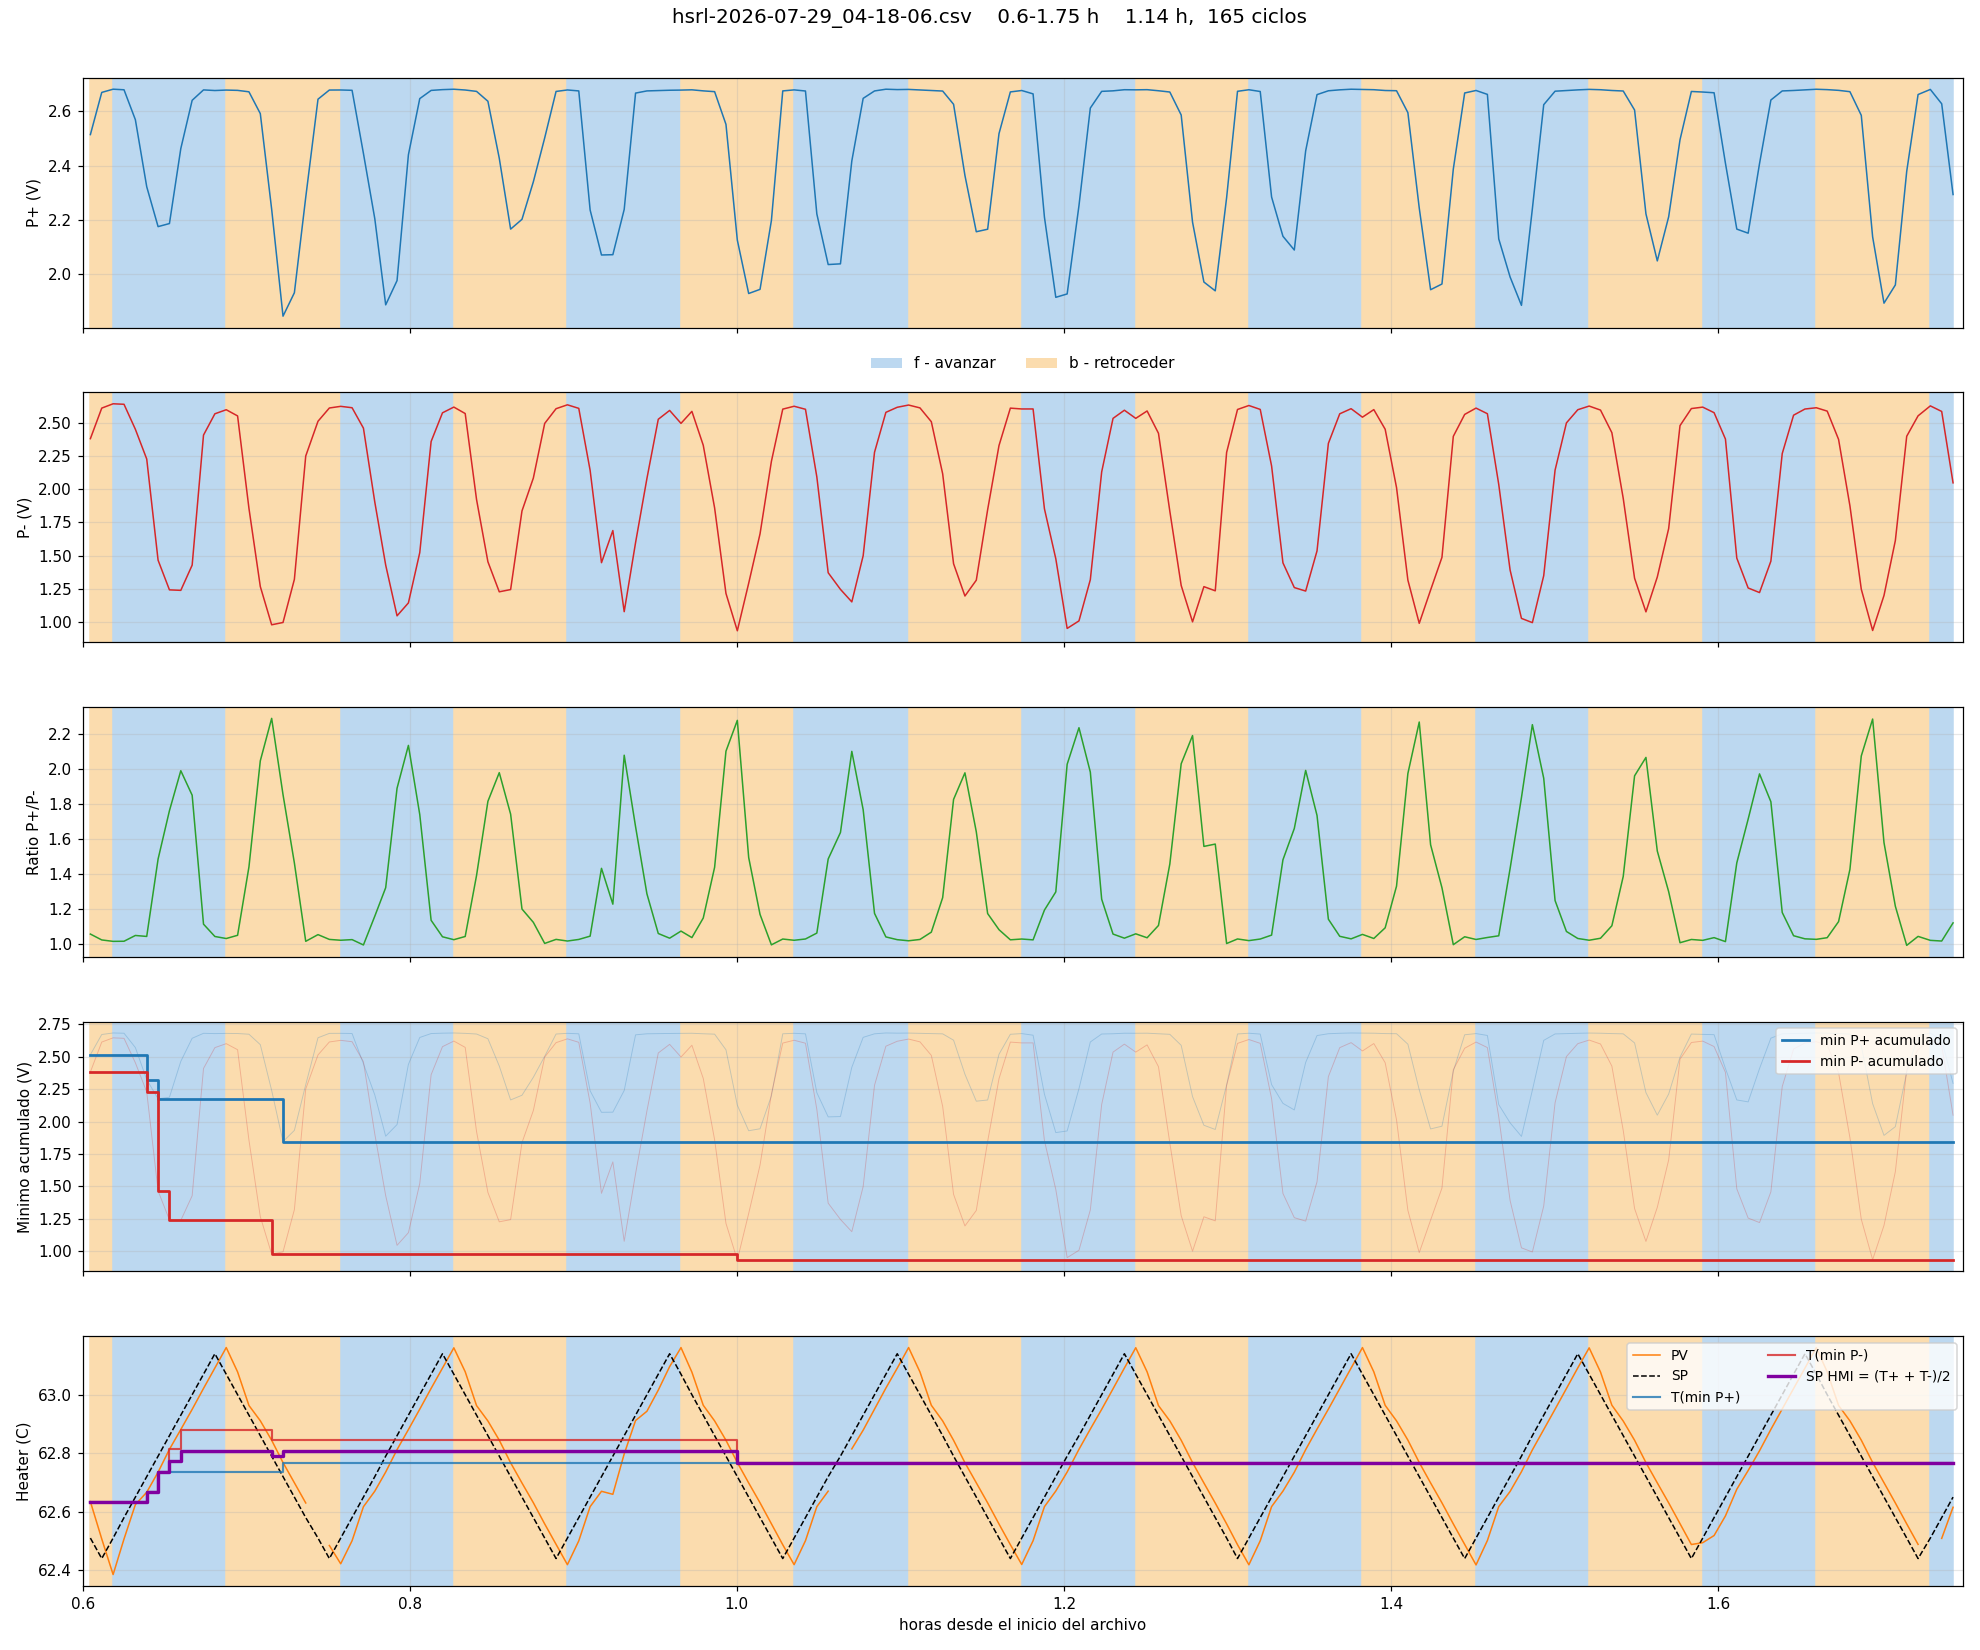
\includegraphics[width=1\textwidth]{figuras/9_sweeps.png}
      \caption{Barridos en temperatura para encontrar punto de operación. El punto de operación aparece luego de 2 horas de barridos (Fuente: elaboración propia).}
      \label{fig:sweep}
\end{figure}

\subsection{Ensayos de estabilidad}

Se realizaron una serie de mediciones de corto plazo para verificar la estabilidad del sistema. Primero se utilizó el instrumento en operación continua, esto es, con el láser disparando a su frecuencia total de $10$~Hz. Las condiciones atmosféricas variaron desde un día despejado hacia un día parcialmente nublado. Para el análisis de la señal lidar se utilizó el código Python almacenado en el repositorio \emph{quicklook} \cite{quicklook}.

La correcta sintonización del instrumento en modo automático se puede visualizar en la Figura~\ref{fig:sintonia}. Para la sintonización, se comandó al equipo a realizar barridos durante un período de 2 horas. Luego de 2 horas, se accionó el comando automático de la HMI. La HMI colocó el punto de trabajo en 62,78\,\textcelsius, definiendo una relación determinada entre $P_+$ y $P_-$. El controlador mediante ajustes finos llevó la temperatura del \emph{seeder} a 62,72\,\textcelsius\ manteniendo la relación entre $P_+$ y $P_-$, \texttt{coe} en el valor definido por la temperatura. 

\begin{figure}[htpb]
      \centering
      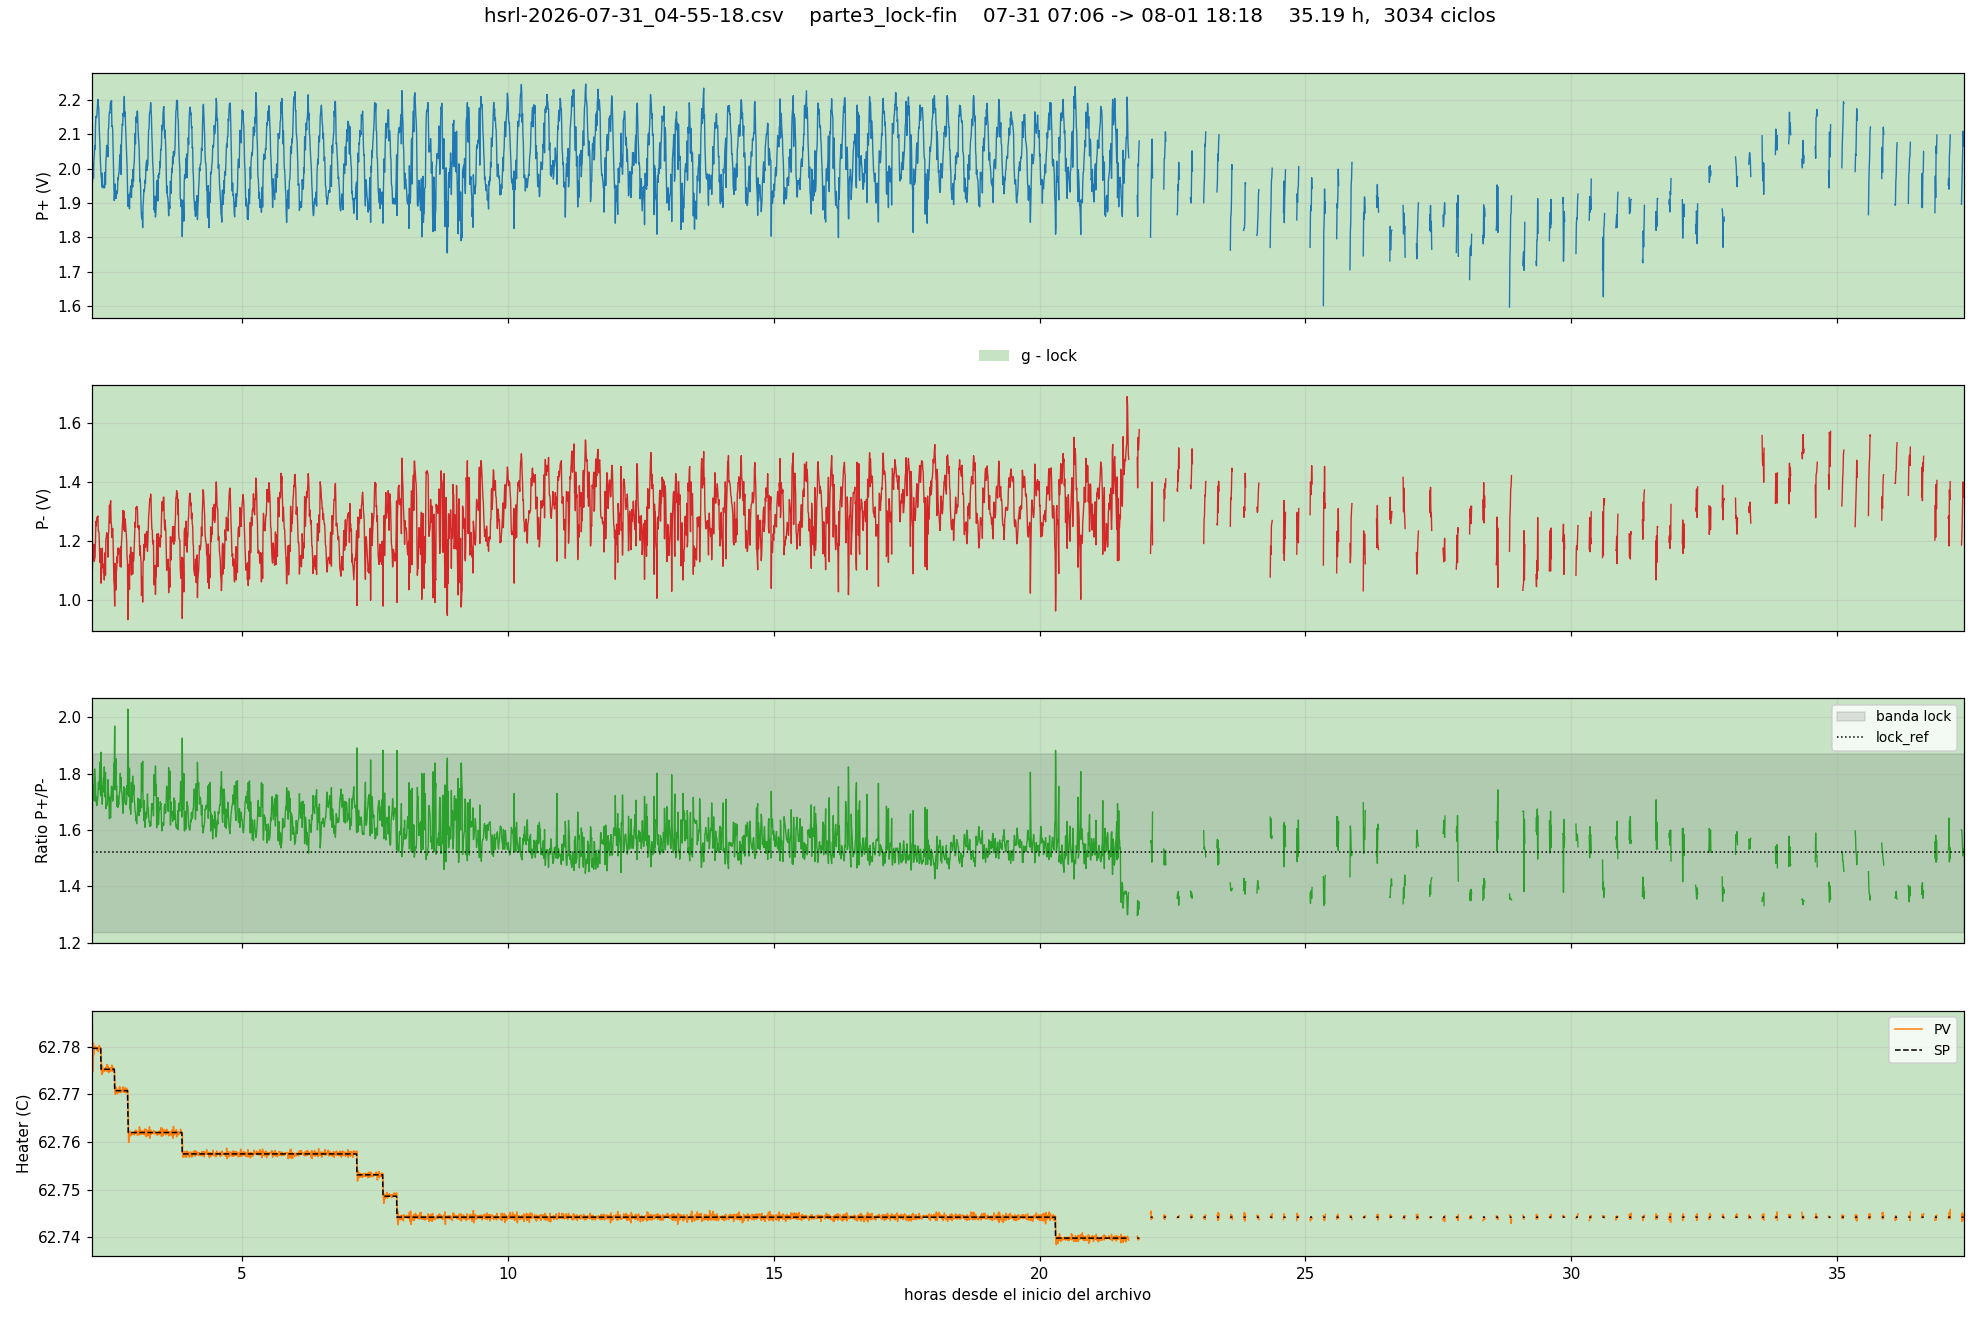
\includegraphics[width=1\textwidth]{figuras/9_sintonía.png}
      \caption{Sintonización del sistema en modo automático (Fuente: elaboración propia).}
      \label{fig:sintonia}
\end{figure}


\begin{figure}[htpb]
      \centering
      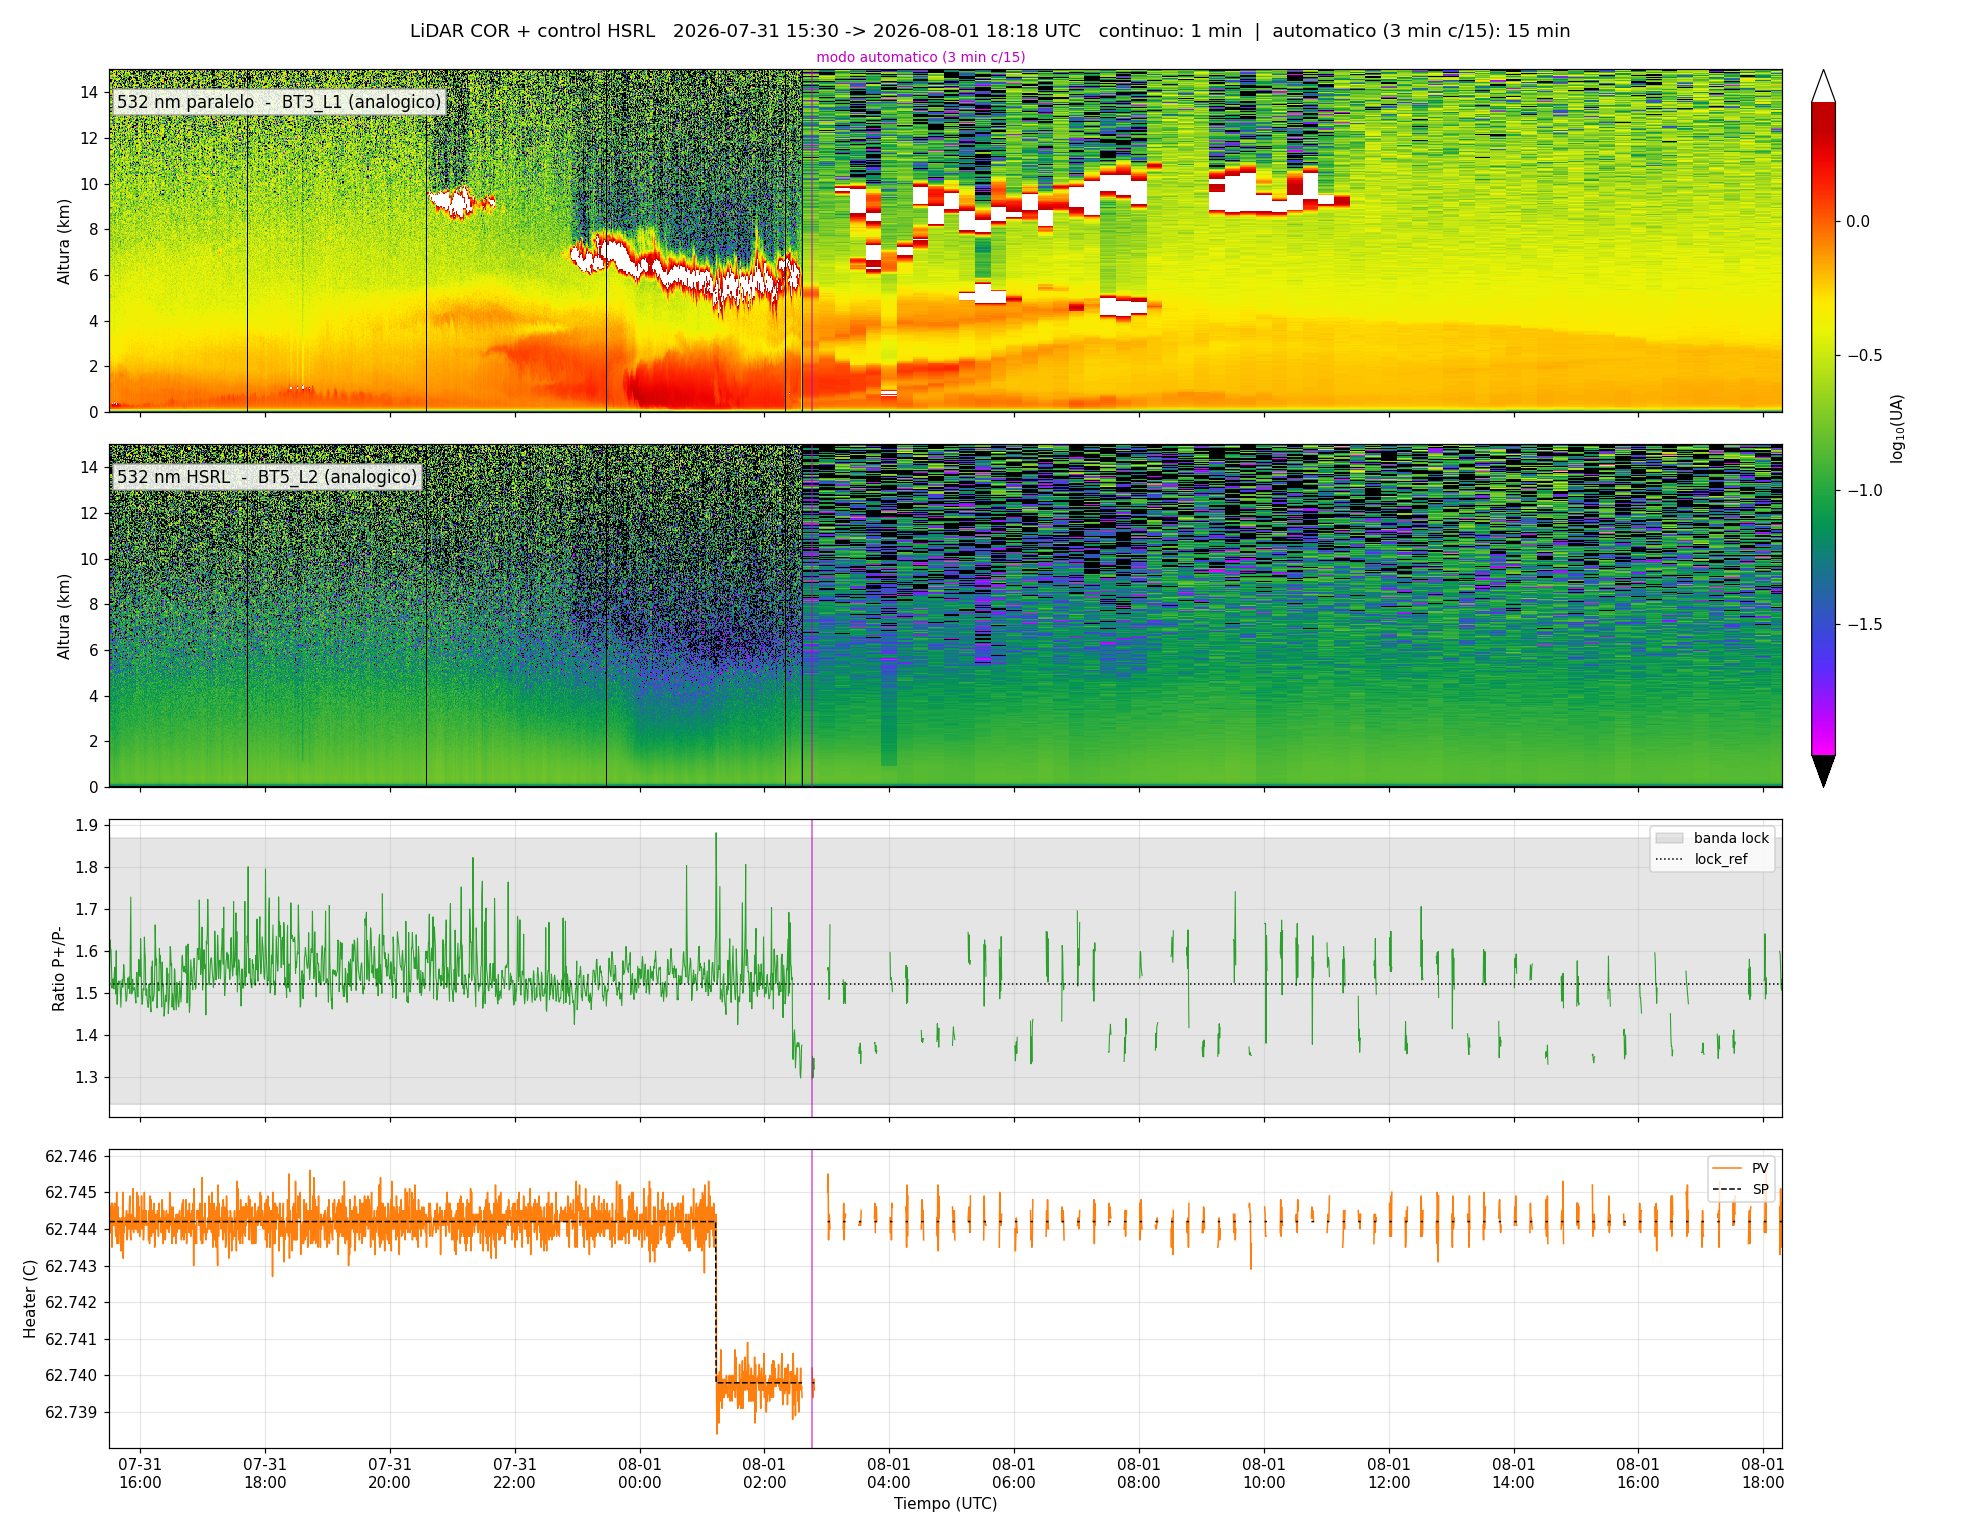
\includegraphics[width=1\textwidth]{figuras/9_autocontinuo.png}
      \caption{Mediciones de atmósfera en canal elástico 532~nm y canal HSR (Fuente: elaboración propia).}
      \label{fig:autocontinuo}
\end{figure}

Luego de tener el sistema sintonizado, se realizaron mediciones de la atmósfera. En la Figura~\ref{fig:autocontinuo} el diagrama de color superior muestra la señal del canal elástico a 532~nm, mientras que el diagrama de color inferior muestra la señal del canal HSR. La diferencia principal entre ambos canales radica en la sensibilidad a la señal retrodispersada por aerosoles. 

Se observan dos evidencias principales que permiten inferir el correcto funcionamiento del canal HSR. La primera es que, ante una fuerte presencia de aerosoles en el rango de 0 a 4 km, el canal HSR muestra una señal mucho más débil que el canal elástico, lo cual es consistente con la teoría de retrodispersión (ya que el canal HSR filtra la componente de los aerosoles). La segunda es que la señal retrodispersada por moléculas a mayor altitud (6 a 10 km) disminuye; esto se debe a la atenuación (extinción) que sufre el haz de luz al atravesar la capa de aerosoles ubicada en los niveles inferiores.

A partir de las 3:00 AM (UTC) el día 01/08/2026, el modo de operación del láser cambia a automático. En este modo, diseñado para preservar la vida útil de la lámpara del láser, el mismo dispara durante 3 minutos cada 15 minutos. Esto se observa en la Figura~\ref{fig:autocontinuo} como franjas horizontales de señal de menor resolución. A pesar de este cambio, el canal HSR sigue mostrando un comportamiento consistente con la teoría de retrodispersión, lo que indica que el lazo de control mantiene la sintonización del láser en la línea de absorción del iodo.

En los últimos dos gráficos de la Figura~\ref{fig:autocontinuo} se observa cómo se mantiene la sintonización del instrumento, realizando un único cambio el día 01/08/2026 a las 2:00 AM (UTC). Esto indica que el lazo de control mantiene la sintonización del láser en la línea de absorción del iodo, incluso cuando el modo de operación del láser cambia a automático. Si bien este análisis se realizó con mediciones cortas, es suficiente para mostrar la correcta sintonización del lazo en modo automático.

\section{Limitaciones conocidas del prototipo}
\label{sec:me-limitaciones}

El modelo descrito constituye un primer prototipo funcional y, como tal, conserva las limitaciones que se detallan a continuación. Su enunciado explícito busca delimitar el alcance de lo validado y orientar una eventual continuidad del trabajo.

\begin{itemize}
  \item El conversor del microcontrolador dispone de canales adicionales y el sistema óptico entrega las señales $P_0$, cuya digitalización podría aportar información al control. El prototipo no las incorpora.
  \item Ante la detección de operación \emph{second mode} el sistema informa la condición pero no descarta la medición ni suspende el lazo, de modo que la corrección queda a cargo del operador.
  \item Para simplificar el primer prototipo no se discriminó entre masa analógica y masa digital. Una revisión posterior de la placa debería evaluar el impacto de esta decisión sobre el piso de ruido de la etapa de detección.
  \item El prototipo no incorpora reguladores de tensión propios, indicadores luminosos ni pulsadores, por lo que depende de la fuente externa y del LED del módulo de desarrollo para la señalización de estado.
  \item Al controlar la temperatura de la celda de iodo mediante un lazo de histéresis, el sistema no puede garantizar una atenuación constante para una determinada temperatura de cavidad de \emph{seeder}. Debido a esto, la banda muerta multiplicativa es del orden del 20\%. Un control más preciso de la temperatura de la celda de iodo permitiría reducir la banda muerta y mejorar la estabilidad del lazo de control.

\end{itemize}